\documentclass{article}

\usepackage{arxiv}
\usepackage[utf8]{inputenc} % allow utf-8 input
\usepackage[T1]{fontenc}    % use 8-bit T1 fonts
\usepackage{hyperref}       % hyperlinks
\usepackage{url}            % simple URL typesetting
\usepackage{booktabs}       % professional-quality tables
\usepackage{amsfonts}       % blackboard math symbols
\usepackage{nicefrac}       % compact symbols for 1/2, etc.
\usepackage{microtype}      % microtypography
\usepackage{lipsum}
\usepackage{graphicx,wrapfig}
\usepackage{caption}
\usepackage{booktabs}
\usepackage{subfig}
\usepackage{float}
\usepackage{wrapfig}
\usepackage{natbib}
\raggedbottom

\title{Diabetic Retinopathy Detection}

\author{
  David Unger\\
  3522491 \\
  Autonome Systeme\\
  University of Stuttgart\\
  \texttt{st172353@stud.uni-stuttgart.de} \\
  \And
  Nick Wagner\\
  3524444 \\
  Autonome Systeme\\
  University of Stuttgart\\
  \texttt{st175644@stud.uni-stuttgart.de} \\
}

% used for confusion matrix
\usepackage{babel}
\usepackage[table]{xcolor}
\usepackage{collcell}
\usepackage{hhline}
\usepackage{pgf}
\usepackage{multirow}
\def\colorModel{hsb} %You can use rgb or hsb
\newcommand\ColCell[1]{
  \pgfmathparse{#1<50?1:0}  %Threshold for changing the font color into the cells
    \ifnum\pgfmathresult=0\relax\color{white}\fi
  \pgfmathsetmacro\compA{0}      %Component R or H
  \pgfmathsetmacro\compB{#1/100} %Component G or S
  \pgfmathsetmacro\compC{1}      %Component B or B
  \edef\x{\noexpand\centering\noexpand\cellcolor[\colorModel]{\compA,\compB,\compC}}\x #1
  } 
\newcolumntype{E}{>{\collectcell\ColCell}m{0.4cm}<{\endcollectcell}}  %Cell width
\newcommand*\rot{\rotatebox{90}}
% end for confusion matrix

\begin{document}
\maketitle

\begin{abstract}
Diabetic retinopathy is an eye disease that can affect people suffering from diabetes. To assist 
doctors and medical personnel with their diagnosis, a classification model shall be trained to classify the severity 
of the disease without human interaction. 
We train and analyze several convolutional neural networks with different architectures. To find an optimal architecture, 
intensive hyperparameter sweeps via random search are performed. We apply different gradient visualization techniques for the performance
analysis of our model.
\end{abstract}

% 1 %%%%%%%%%%%%%%%%%%%%%%%%%%%%%%%%%%%%%%%%%%%%%%%%%%%%%%%%%%%%%%%%%%%%%%%%%%%%%%%%%%%%%%%%%%%%%%%%%%%%%%%%%%%%%%%%%%%%%%
\section{Introduction}
Diabetic retinopathy is a complication of diabetes, which can cause damage to the retina of the eye.
To treat this condition successfully, it has to be detected at an early stage, which is difficult due to minimal or no early warning signs. 
Furthermore, the different grades can only be distinguished by a trained professional due to its subtle symptoms.
Examples for those are leaking blood vessels, fatty deposits or retinal swelling.
Since this task is difficult even for trained professionals \cite{DBRscience}, the goal of this paper is to find an algorithm for automatic
detection of the diabetic retinopathy grade. The dataset is the Indian Diabetic Retinopathy Image Dataset (IDRID), which 
is publicly available \cite{IDRiDdataset}. It contains five class labels, which refer to each of the eye disease grades (0-4).

% 2 %%%%%%%%%%%%%%%%%%%%%%%%%%%%%%%%%%%%%%%%%%%%%%%%%%%%%%%%%%%%%%%%%%%%%%%%%%%%%%%%%%%%%%%%%%%%%%%%%%%%%%%%%%%%%%%%%%%%%%
\section{Object Classification}
\subsection{Problem analysis}

To tackle the problem of diabetic retinopathy detection, several methods are possible. Because the dataset consists of 
ordinally scaled data of 5 classes, regression could be used to estimate the severity of a case. In addition, the problem 
can be handled as a binary or multiclass classification problem after one-hot-encoding the labels.
Further, only binary and multiclass classification are analyzed.

A binary classification has the advantage of higher accuracy, but lacks details, because the network doesn't output 
information about the exact severity of the disease. Metrics are easy to implement because precision, 
recall and F1-score are standard implementations and nicely interpretable. A multiclass classification has typically a 
lower accuracy, because the network needs to pick the right class among 
several classes. It provides the benefit of receiving richer information, i.e. the exact severity of the disease.
Evaluating a multiclass classification problem becomes harder, because misclassifications can vary in their error.

\subsection{Architecture}
To tackle the classification problem, we train several neural networks using different architectures.
The analyzed model architectures are composed of three parts: the 
base model, the conversion layer and the head of our model. For the base model we try both ResNet50 and VGG16 with 
weights pretrained on ImageNet. We evaluate the results with a fully trainable, partly trainable and not trainable
base model. As conversion layer we test both, a flatten and global average pooling (GAP) layer.
For the head we try up to three hidden dense layers with different numbers of neurons per layer.
The final output consists of five values that correspond to the five diabetic retinopathy grade predictions, see Figure \ref{fig:architecture}.
The decision for this architecture is based on parameter optimization of many factors which get discussed in chapter \ref{ch_hyperparam}.

\begin{figure}[h]
  \centering
  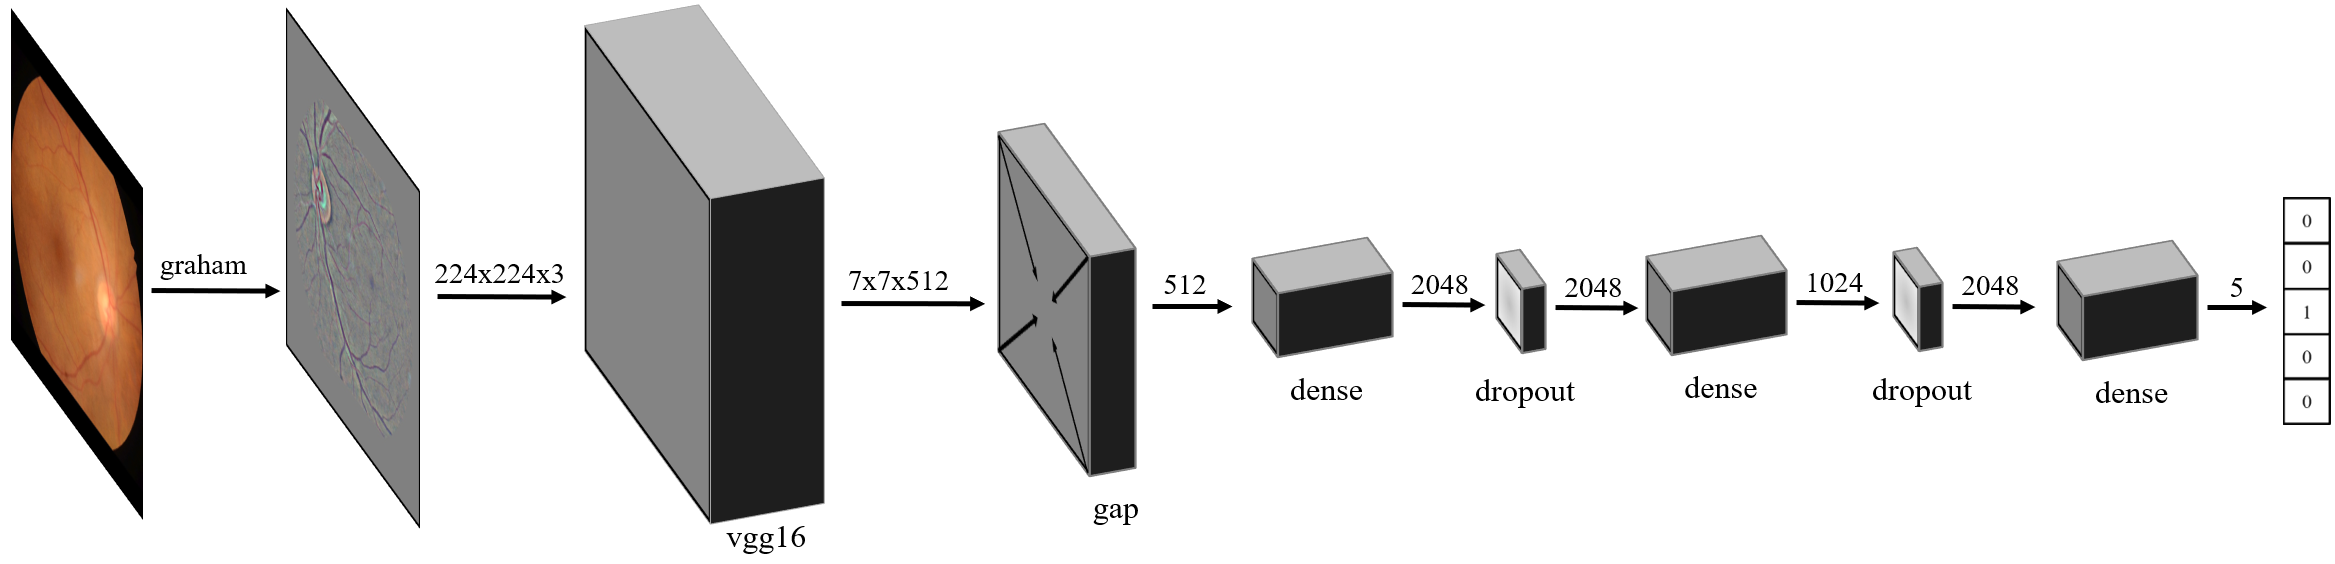
\includegraphics[width=1\textwidth]{2_2_architecture.png}\label{fig:architecture}
  \caption{Final model architecture}
  \label{fig:architecture}
\end{figure}

\subsection{Weight initialization}
Weight initialization refers to the initial values of parameters that are used in neural network layers.
Changing the initialization of the layers changes the starting point for the optimization process and potentially also the performance.
Keras initializes the weights of dense layers with the Glorot uniform initializer, which draws samples from a truncated uniform distribution.
Generally the goal is to avoid vanishing and exploding gradients, even better is if the variance of layer outputs is approximately one. \cite{kumar2017weight}
Specifically for the ReLU activation function, this is achieved with the He initialization, which draws from a normal distribution with the following parameters. \cite{he2015delving}\\
%\begin{minipage}{.5\linewidth}
  \begin{equation}
    \mu = 0
  \end{equation}
%\end{minipage}
%\begin{minipage}{.5\linewidth}
  \begin{equation}
    \sigma^2 = 2/N
  \end{equation}
%\end{minipage}

\subsection{Augmentation}
\begin{wrapfigure}{r}{6cm}%[h]
  \vspace{-10pt}
  \centering
  \subfloat[Original image]{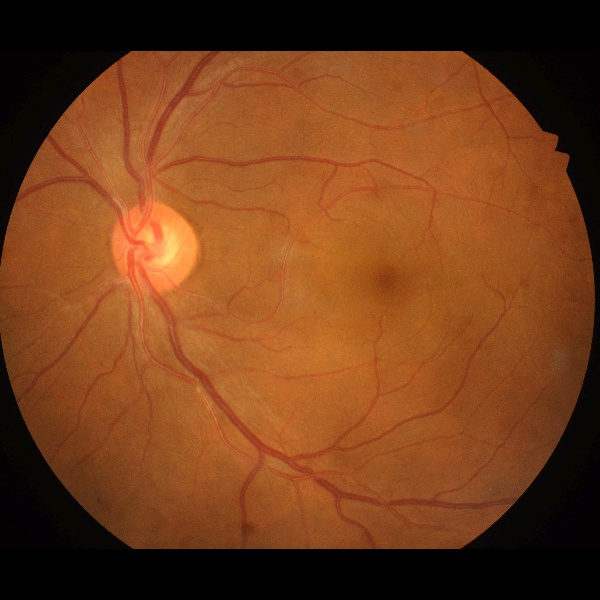
\includegraphics[width=0.15\textwidth]{IDRiD_060.jpg}\label{fig:IDRiD_backprop_orig}}
  \hspace{0.5cm}
  \subfloat[Processed image]{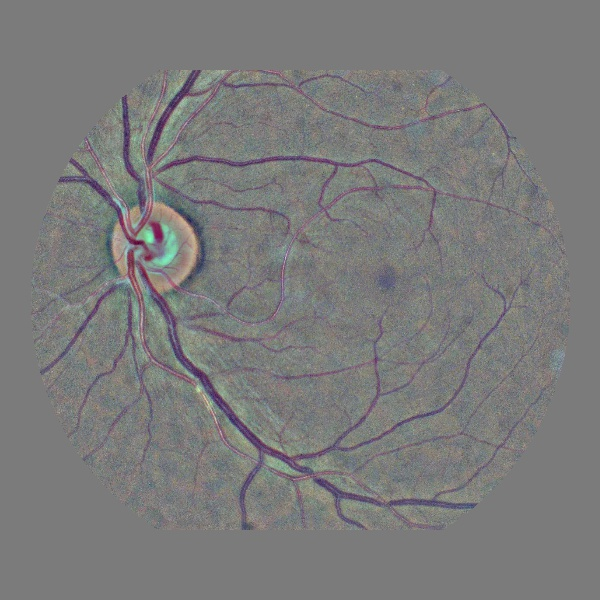
\includegraphics[width=0.15\textwidth]{IDRiD_060_graham.jpg}\label{fig:IDRiD_backprop_enh}}
  \caption{Graham preprocessing}
  \label{fig:graham}
\end{wrapfigure}
Within the input pipeline three main types of augmentation are applied.
The goal is to make feature extraction easier for the network and increase the amount of input images which reduces overfitting.
\begin{itemize}
  \item[-] \textbf{Graham preprocessing:}\cite{graham2015} see Figure \ref{fig:graham}\begin{itemize}
    \item[1.] rescale the eye radius to 300 pixels 
    \item[2.] subtract the local average color (Gaussian blur) 
    \item[3.] shift the value of the difference image by 128
    \item[4.] clip the image to remove boundary effects
  %   \begin{figure}[h]
  %     \begin{minipage}[b]{.5\textwidth}
  %         \begin{center}
  %         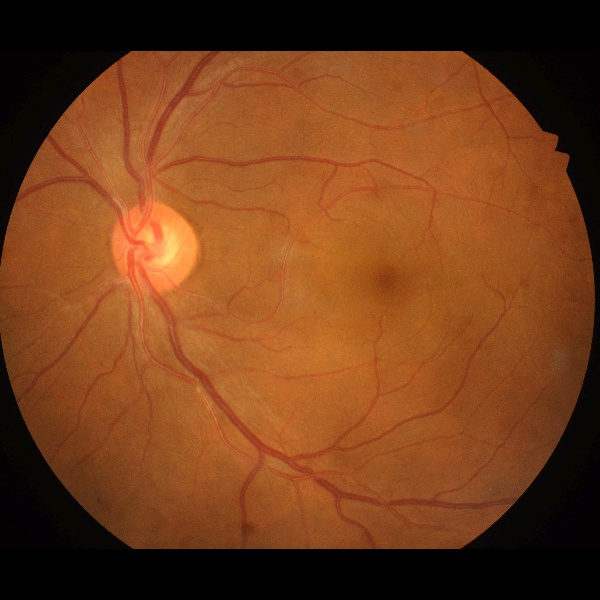
\includegraphics[width=.5\linewidth]{IDRiD_060.jpg}
  %         \captionsetup{justification=centering}
  %         \captionof{figure}{Original image}
  %         \label{fig:IDRiD}
  %         \end{center}
  %     \end{minipage}%
  %     \begin{minipage}[b]{.5\textwidth}
  %         \begin{center}
  %         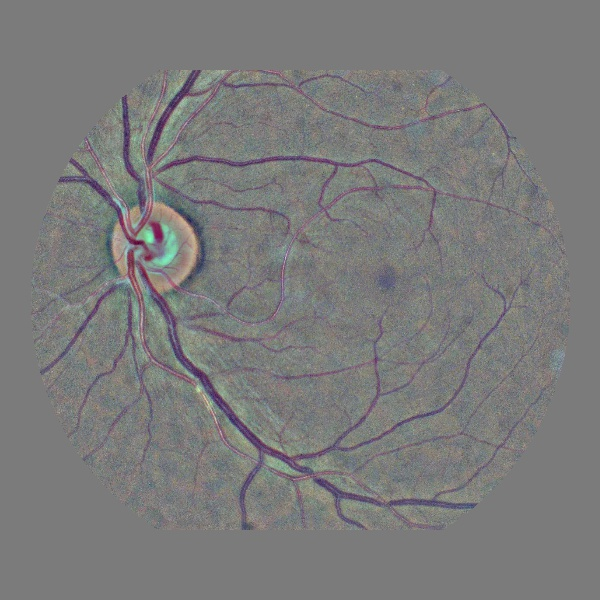
\includegraphics[width=.5\linewidth]{IDRiD_060_graham.jpg}
  %         \captionsetup{justification=centering}
  %         \captionof{figure}{Graham preprocessed image}
  %         \label{fig:IDRiD_graham}
  %         \end{center}
  %     \end{minipage}
  % \end{figure} 
  \end{itemize}   
  \item[-] \textbf{Color jittering:} Slight random changes to brightness, hue, saturation and contrast.
  \item[-] \textbf{Random cropping:} Crop a window that is slightly smaller than the image. Then resize to original image size again.
\end{itemize}

% Dataset Balancing
\subsection{Dataset Balancing}
\renewcommand{\arraystretch}{1.2}
\begin{wraptable}{r}{6cm}
  \vspace{-15pt}
  \centering
  \begin{tabular}{|l|l|l|l|l|l|}
  \hline
  Label:   & 0   & 1  & 2   & 3  & 4  \\ \hline \hline
  \# train & 134 & 20 & 136 & 74 & 49 \\ \hline
  \# test  & 34  & 5  & 32  & 19 & 13 \\ \hline
  \end{tabular}
  \caption{Dataset sample distribution} \label{tab:table1}
  \end{wraptable}
Taking a closer look at the sample distribution within the dataset as shown in Table \ref{tab:table1}, it is obviously imbalanced. This will inevitably lead to a trained model
that is fitted better to the overrepresented classes.
To avoid this, a method called oversampling is applied. Oversampling allows drawing underrepresented classes from the training set more often, 
such that all classes are equally represented when training the model.
\pagebreak
\subsection{Training \& Metrics}
For training our model, we use categorical cross-entropy as loss function and experiment with the optimizer and 
learning rate. As optimizer we select SGD with a momentum of 0.9 and Adam which both show similar performance. 
As learning rate, we use 0.1, 0.01 and 0.001 from which the latter performs best. Further learning rate decay
shows no improvement.

Training deep neural networks requires some performance metrics indicating the success or failure of the model fitting. Accuracy
is easy to understand and to implement, but not suited for imbalanced data, because it doesn't take into account how well each 
single class is predicted. 
To overcome this, precision (how accurate the model is with its prediction) and recall (how thorough the model is with its prediction) can be used. 
Especially a combination of both, the F1-score is a metric that indicates how well a classifier handles different classes.

For the diabetic retinopathy dataset, the F1-score comes with a drawback. The dataset has ordinal labels, which means predicting 
a wrong class is not equally bad. As an example, predicting class 0 (no retinopathy) for the true class 4 (proliferative retinopathy) 
is much worse than predicting class 3 (severe retinopathy). The F1-score counts both misclassifications equally, while the 
Quadratic Weighted Kappa (QWC) metric takes the distance of the classification error into account and is therefore more suitable \cite{QWC}.
% 3 %%%%%%%%%%%%%%%%%%%%%%%%%%%%%%%%%%%%%%%%%%%%%%%%%%%%%%%%%%%%%%%%%%%%%%%%%%%%%%%%%%%%%%%%%%%%%%%%%%%%%%%%%%%%%%%%%%%%%%
\section{Experiments}
\subsection{Procedure}
The training of the deep neural network classifier requires the selection of suitable hyperparameters that differ from
problem to problem, which is why their choice is a hard task. A useful strategy to find a good set of hyperparameters are parameter 
sweeps. Weights\&Biases is a Python library that enables the easy implementation of sweeps and is therefore selected for our implementation. 

Hyperparameter optimization requires besides the training and test dataset a third, the validation dataset, to evaluate the
model after hyperparameter tuning and to avoid overfitting on the hyperparameters. Because the given dataset only contains 
training and test data, the original training dataset is split into 80\% training data and 20\% validation data.
To perform many parameter sweeps, we store our dataset in the cloud and use Google Colab as training server. 

\subsection{Hyperparameter selection}\label{ch_hyperparam}


\renewcommand{\arraystretch}{1.2}
\begin{wraptable}{r}{7.5cm}
  \vspace{-20pt}
  \begin{tabular}{|l|l|}
  \hline
  Hyperparameter & Selected\\ \hline \hline
  Model architecture & ResNet50 \\ \hline
  Learning rate & 0.001 \\ \hline
  Balancing & true \\ \hline
  Flatten or GAP & GAP \\ \hline
  Number of dense neurons in layer N-3 & 4096 \\ \hline
  Number of dense neurons in layer N-2 & 512 \\ \hline
  Number of dense neurons in layer N-1 & 0 \\ \hline
  \end{tabular}
  \caption{Excerpt of the most important hyperparameters} \label{tab:hyperparam}
  \end{wraptable}


As metrics for hyperparameter selection, we mainly use correlation with the validation-QWC-score and 
compare the minimum, median and maximum run of each sweeped hyperparameter value with each other. 
Once most important hyperparameter is determined and selected, one needs to ensure that the second most important
parameter is not selected because of strong correlation with the most important one. This independence can be 
guaranteed by filtering the sweep and selecting just runs with the best parameter or by performing a new parameter sweep
with having this first parameter fixed.

Following this procedure, we select the most important hyperparameters as in Table \ref{tab:hyperparam}.



%\begin{figure}[h]
%  \centering
%  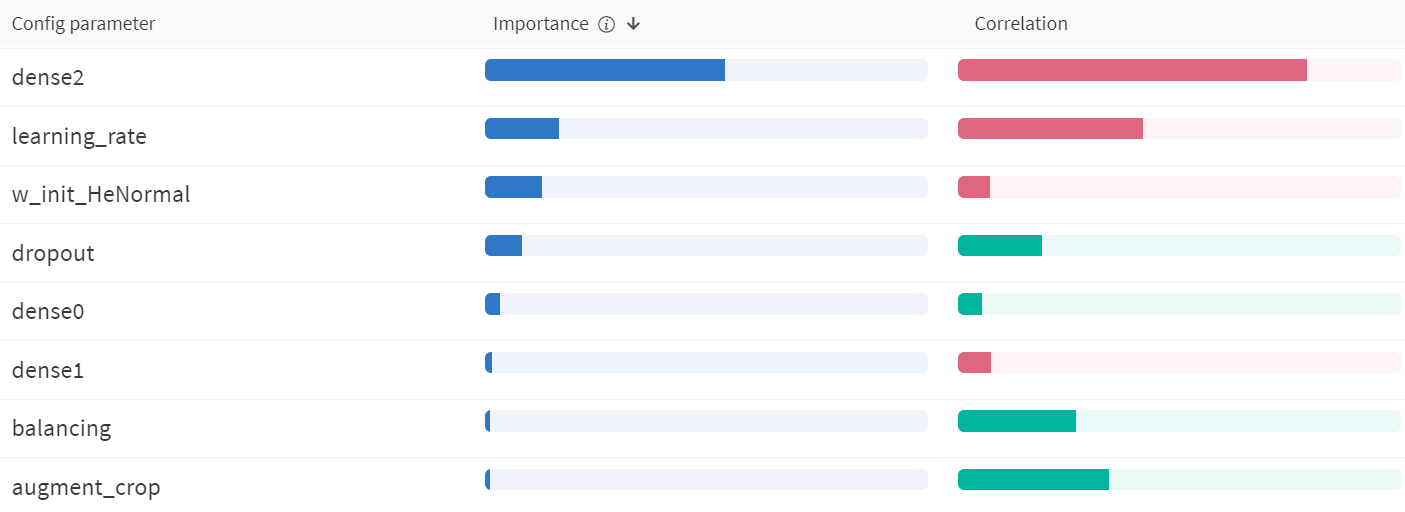
\includegraphics[width=0.8\textwidth]{3_2_parameter_importance.png}\label{fig:param_importance}
%  \caption{Most important parameters with a sweep of 80 experiments}
%\end{figure}


% Deep Visualization
\subsection{Deep Visualization}
\subsubsection{Guided Backpropagation}
\begin{wrapfigure}{r}{7cm}%[h]
  \vspace{-50pt}
  \centering
  \subfloat[Original result]{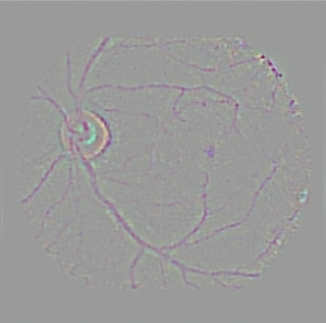
\includegraphics[width=0.15\textwidth]{IDRiD_060_backprop_orig.png}\label{fig:IDRiD_backprop_orig}}
  \hspace{0.5cm}
  \subfloat[Enhanced result]{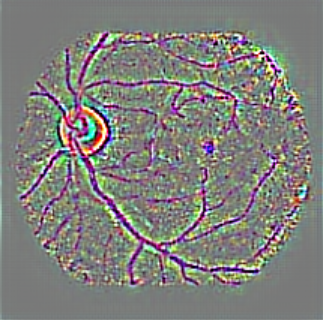
\includegraphics[width=0.15\textwidth]{IDRiD_060_backprop_enh.png}\label{fig:IDRiD_backprop_enh}}
  \caption{Guided Backpropagation}
  \label{guidedBackprop}
\end{wrapfigure}
Guided Backpropagation\cite{springenberg2015striving} belongs to the family of pixel-space gradient visualizations. 
The goal is to exploit the idea that neurons act like detectors of image features by using backpropagation.
What makes this backpropagation guided is that negative gradients are set to zero. This way, only pixels that are positively impacting 
the output get highlighted. This method is not class-discriminative. See Figure \ref{guidedBackprop} and \ref{deepVis}a.
\subsubsection{CAM}
Class Activation Map (CAM)\cite{ZhouKLOT15} is class-discriminative and highlights relevant image regions, but in a less fine-grained manner.
To achieve this, global average pooling has to be performed on the feature maps of the last convolutional layer, followed by a dense layer as output.
The weights of this dense layer are then projected back to the convolutional feature maps which results in the class activation mappings.
As a consequence, it is hard to generalize this approach due to the architecture restrictions.
\subsubsection{GradCAM}
GradCAM\cite{SelvarajuDVCPB16} is class-discriminative as well, but can be used by any CNN-based network without architectural adaptations.
Similar to CAM, it describes the activation as a linear combination of weighted feature maps. But in this case, the weights are calculated
by deriving the respective logit of the class of interest by the feature maps of the chosen convolutional layer. These gradients then get global average pooled, followed by a ReLU.
The ReLU leaves only feature with a positive impact behind, similar to how it is applied in Guided Backpropagation. See Figure \ref{deepVis}b.
\subsubsection{Guided GradCAM}
Guided GradCAM\cite{SelvarajuDVCPB16} combines the ideas of Guided Backpropagation with Class Activation Maps.
This makes GradCAM class-discriminative due to the localization of relevant image regions and high-resolution due pixel-space gradient visualization. See Figure \ref{deepVis}c.
\begin{figure}[H]
  \centering
  \subfloat[Guided Backprop.]{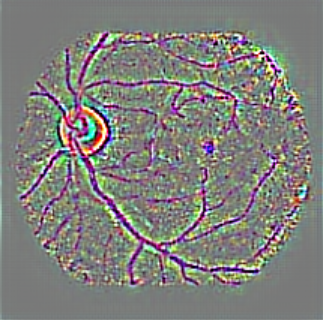
\includegraphics[width=0.2\textwidth]{IDRiD_060_backprop_enh.png}\label{fig:IDRiD_backprop_orig}}
  \hspace{0.5cm}
  \subfloat[gradCAM]{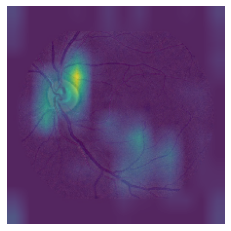
\includegraphics[width=0.2\textwidth]{IDRiD_060_gradCAM.png}\label{fig:IDRiD_backprop_enh}}
  \hspace{0.5cm}
  \subfloat[Guided gradCAM]{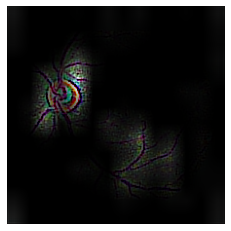
\includegraphics[width=0.2\textwidth]{IDRiD_060_guided_gradCAM.png}\label{fig:IDRiD_backprop_enh}}
  \caption{Deep Visualization result example}
  \label{deepVis}
\end{figure}

% 4 %%%%%%%%%%%%%%%%%%%%%%%%%%%%%%%%%%%%%%%%%%%%%%%%%%%%%%%%%%%%%%%%%%%%%%%%%%%%%%%%%%%%%%%%%%%%%%%%%%%%%%%%%%%%%%%%%%%%%%
\section{Results}



\begin{wraptable}{r}{6.5cm} % start confusion matrix
  \centering
  \newcommand\items{5}   %Number of classes
  \arrayrulecolor{white} %Table line colors
  \noindent\begin{tabular}{cc*{\items}{|E}|}
    \multicolumn{1}{c}{} &\multicolumn{1}{c}{} &\multicolumn{\items}{c}{Predicted} \\ \hhline{~*\items{|-}|}
    \multicolumn{1}{c}{} & 
    \multicolumn{1}{c}{} & 
    \multicolumn{1}{c}{\rot{Class 0}} & 
    \multicolumn{1}{c}{\rot{Class 1}} & 
    \multicolumn{1}{c}{\rot{Class 2}} & 
    \multicolumn{1}{c}{\rot{Class 3}} & 
    \multicolumn{1}{c}{\rot{Class 4}} \\ \hhline{~*\items{|-}|}
    \multirow{\items}{*}{\rotatebox{90}{True}} 
    &Class 0  & 29 &  2 &  2 &  0 &  1   \\ \hhline{~*\items{|-}|}
    &Class 1  &  0 &  3 &  2 &  0 &  0   \\ \hhline{~*\items{|-}|}
    &Class 2  &  7 &  1 & 15 &  3 &  6   \\ \hhline{~*\items{|-}|}
    &Class 3  &  2 &  0 &  3 &  9 &  4   \\ \hhline{~*\items{|-}|}
    &Class 4  &  4 &  0 &  1 &  1 &  7   \\ \hhline{~*\items{|-}|}
  \end{tabular}
  \vspace{0.2cm}
  \caption{Confusion matrix on the test dataset}
  \label{tab:confm}
  \end{wraptable} % end confusion matrix
We train and evaluate our algorithm on both binary and multiclass classification.

For binary classification we perform a hyperparameter sweep and achieve without further optimization an F1-score of 0.87 on the 
validation data and of 0.82 on the test data.

For multiclass classification we optimize our model further and perform several sweeps. Our finally selected model achieves 
an accuracy of 58.8\%, an F1-score of 0.47 and a QWC score of 0.44 which would have achieved rank 106 for the Kaggle challenge. 
When evaluating the confusion matrix of the prediction as denoted in Table \ref{tab:confm}, one can see that our model predicts
class 0 very frequently and often incorrectly. This can be interpreted in a way that our model fails to identify features that
indicate the disease and therefore selects class 0. As a result, our model could be further optimized by more extensive data augmentation 
like shearing or rotating the images to overcome the challenge of a relatively small dataset.


\bibliographystyle{unsrt}  
%\bibliography{references}  %%% Remove comment to use the external .bib file (using bibtex).
%%% and comment out the ``thebibliography'' section.

%%% Comment out this section when you \bibliography{references} is enabled.
\begin{thebibliography}{1}

  \bibitem{DBRscience}
  Goh, James Kang H.; Cheung, Carol Y.; Sim, Shaun S.; Tan, Pok C.; Tan, Gavin Siew W.; Wong, Tien Y.
  \newblock Retinal imaging techniques for diabetic retinopathy screening.
  \newblock {\em Journal of diabetes science and technology 10}, 2016.

  \bibitem{IDRiDdataset}
  Porwal, Prasanna; Pachade, Samiksha; Kamble, Ravi; Kokare, Manesh; Deshmukh, Girish; Sahasrabuddhe, Vivek; Meriaudeau, Fabrice.
  \newblock Indian diabetic retinopathy image dataset (IDRiD): a database for diabetic retinopathy screening research.
  \newblock {\em Data 3}, 2018.

  \bibitem{kumar2017weight}
  Kumar, Siddharth Krishna.
  \newblock On weight initialization in deep neural networks.
  \newblock {\em arXiv:1704.08863}, 2017.

  \bibitem{he2015delving}
  He, Kaiming; Zhang, Xiangyu; Ren, Shaoqing; Sun, Jian.
  \newblock Delving Deep into Rectifiers: Surpassing Human-Level Performance on ImageNet Classification.
  \newblock {\em arXiv:1502.01852}, 2015.

  \bibitem{graham2015}
  Graham, Benjamin.
  \newblock Diabetic retinopathy Kaggle challenge report.
  \newblock {\em https://www.kaggle.com/c/diabetic-retinopathy-detection/discussion/15801}, 2015.

  \bibitem{QWC}
  Cohen, Jacob. 
  \newblock Weighted kappa: Nominal scale agreement provision for scaled disagreement or partial credit. 
  \newblock Psychological Bulletin, 70(4), 213–220, 1968. 
  
  \bibitem{springenberg2015striving}
  Springenberg, Jost Tobias; Dosovitskiy, Alexey; Brox, Thomas; Riedmiller, Martin.
  \newblock Striving for Simplicity: The All Convolutional Net.
  \newblock {\em arXiv:1412.6806}, 2015.

  \bibitem{ZhouKLOT15}
  Zhou, Bolei; Khosla, Aditya; {\`{A}}gata, Lapedriza; Aude Oliva; Antonio, Torralba.
  \newblock Learning Deep Features for Discriminative Localization.
  \newblock {\em arXiv:1512.04150}, 2015.

  \bibitem{SelvarajuDVCPB16}
  Ramprasaath R., Selvaraju; Abhishek, Das; Ramakrishna, Vedantam; Michael, Cogswell; Devi, Parikh; Dhruv, Batra.
  \newblock Grad-CAM: Why did you say that? Visual Explanations from Deep Networks via Gradient-based Localization.
  \newblock {\em arXiv:1610.02391}, 2016.

  \end{thebibliography}



\end{document}
